
\documentclass{article} % For LaTeX2e
\usepackage{icais2025_conference,times}

% Optional math commands from https://github.com/goodfeli/dlbook_notation.
\input{math_commands.tex}

\usepackage{hyperref}
\input{math_commands.tex}
\usepackage{url}
\usepackage{graphicx}
\usepackage{subfigure}
\usepackage{booktabs}

% For theorems and such
\usepackage{amsmath}
\usepackage{amssymb}
\usepackage{mathtools}
\usepackage{amsthm}

% Custom
\usepackage{multirow}
\usepackage{color}
\usepackage{colortbl}
\usepackage[capitalize,noabbrev]{cleveref}
\usepackage{xspace}
\hypersetup{
    colorlinks=true,
    linkcolor=blue!70!black,
    citecolor=green!60!black,
    urlcolor=red!60!black
}
\usepackage{url}


\title{Exploring Creative Limits of Language Models through Multi-Token Prediction and Seed-Conditioning}

% Authors must not appear in the submitted version. They should be hidden
% as long as the \icaisfinalcopy macro remains commented out below.
% Non-anonymous submissions will be rejected without review.

\author{Antiquus S.~Hippocampus, Natalia Cerebro \& Amelie P. Amygdale \thanks{ Use footnote for providing further information
about author (webpage, alternative address)---\emph{not} for acknowledging
funding agencies.  Funding acknowledgements go at the end of the paper.} \\
Department of Computer Science\\
Cranberry-Lemon University\\
Pittsburgh, PA 15213, USA \\
\texttt{\{hippo,brain,jen\}@cs.cranberry-lemon.edu} \\
\And
Ji Q. Ren \& Yevgeny LeNet \\
Department of Computational Neuroscience \\
University of the Witwatersrand \\
Joburg, South Africa \\
\texttt{\{robot,net\}@wits.ac.za} \\
\AND
Coauthor \\
Affiliation \\
Address \\
\texttt{email}
}

% The \author macro works with any number of authors. There are two commands
% used to separate the names and addresses of multiple authors: \And and \AND.
%
% Using \And between authors leaves it to \LaTeX{} to determine where to break
% the lines. Using \AND forces a linebreak at that point. So, if \LaTeX{}
% puts 3 of 4 authors names on the first line, and the last on the second
% line, try using \AND instead of \And before the third author name.

\newcommand{\fix}{\marginpar{FIX}}
\newcommand{\new}{\marginpar{NEW}}

%\iclrfinalcopy % Uncomment for camera-ready version, but NOT for submission.
\begin{document}


\maketitle

\begin{abstract}
This research introduces a controlled set of minimal algorithmic tasks that evaluate the creative limits of large language models (LLMs). These tasks require a stochastic planning step that either discovers novel connections in knowledge graphs or constructs new patterns, simulating open-ended real-world challenges. We propose that traditional next-token learning is myopic, whereas multi-token prediction (MTP) approaches, such as teacherless training and diffusion models, excel in producing diverse and original outputs. Our novel seed-conditioning technique, which introduces randomness at the input layer, is presented as an effective method to elicit creativity without sacrificing coherence, performing comparably to existing output-layer temperature sampling. This study aims to provide a principled framework for assessing the creative capabilities of LLMs and advocates for a shift away from conventional next-token learning paradigms.
\end{abstract}

\section{Introduction}
\label{sec:intro}
The creative limits of language models (LLMs) remain inadequately explored, particularly in tasks necessitating abstract reasoning. Traditional next-token prediction methods often fall short when faced with open-ended challenges requiring innovative thinking. This research investigates the potential of multi-token prediction (MTP) and seed-conditioning to enhance the algorithmic creativity of LLMs. By allowing models to predict multiple tokens simultaneously, we hypothesize that these approaches may facilitate the generation of more creative and diverse outputs compared to conventional methods. The primary contributions of this study include the introduction of a novel task suite designed to evaluate creativity and the implementation of seed-conditioning to enhance model outputs through controlled randomness.

\section{Related Work}
\label{sec:related}
Prior research has established that MTP can significantly improve the performance of LLMs in various contexts \citep{kalinsky2023simpleae, walker2024futuretp}. However, studies specifically quantifying the creative limits of LLMs in open-ended scenarios remain sparse. The concept of seed-conditioning, which introduces randomness at the input level, parallels techniques such as adaptive temperature sampling \citep{zhu2023hotoc}, and the Burn Layer \citep{hassan2024optimizingpa}. This research adds to the existing literature by focusing on a structured test-bed for assessing creativity and the unique application of seed-conditioning in this context.

\section{Method}
\label{sec:method}
We developed a series of algorithmic tasks that necessitate creative leaps, such as generating analogies and solving complex problems. The LLMs were trained using both traditional next-token prediction and MTP combined with seed-conditioning. The latter method introduces variability at the input layer, enhancing the model's ability to explore diverse outputs. Our approach aims to balance the need for coherence with the desire for creativity, positioning seed-conditioning as a viable alternative to established randomness methods.

\section{Experimental Setup}
\label{sec:experimental_setup}
We designed experiments to compare the outputs of LLMs trained with different methodologies. Metrics for evaluating creativity included N-gram diversity, novelty scores, and human evaluations. The training involved varying dropout rates in an LSTM model, using synthetic datasets to gauge the impact on the Creative Output Distinctiveness Score (CODS) and training loss.

\section{Experiments}
\label{sec:experiments}
The experiments yielded insights into model performance across multiple configurations. Figure \ref{fig:loss_cods} illustrates the training loss and CODS over epochs for the baseline dropout tuning experiment. The results showed fluctuations in the CODS metric, indicating instability, while the training loss demonstrated a steady decrease with occasional spikes.

\begin{figure}[h!]
    \centering
    \subfigure[Training Loss over Epochs]{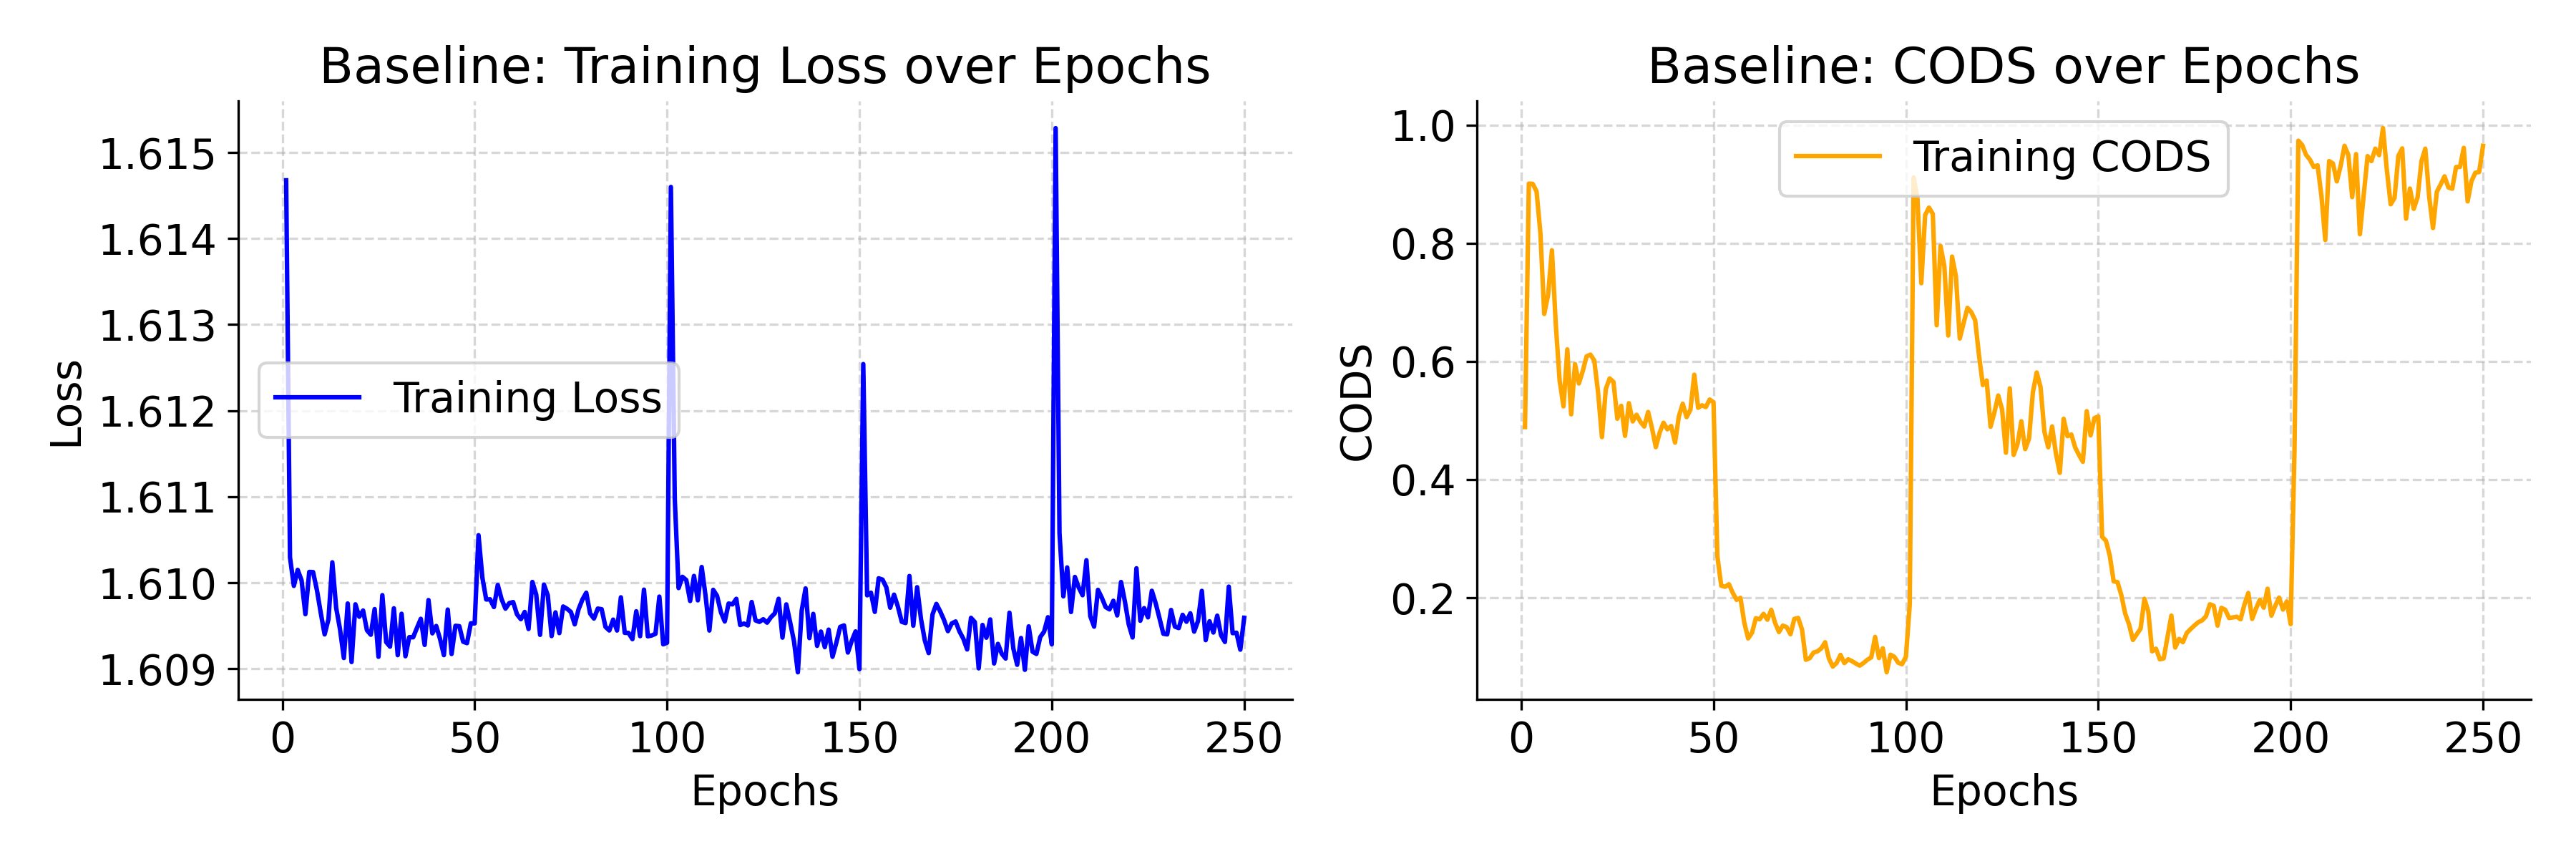
\includegraphics[width=\textwidth]{img/baseline_dropout_tuning.png}}
    \hspace{0.5cm}
    \subfigure[Training CODS over Epochs]{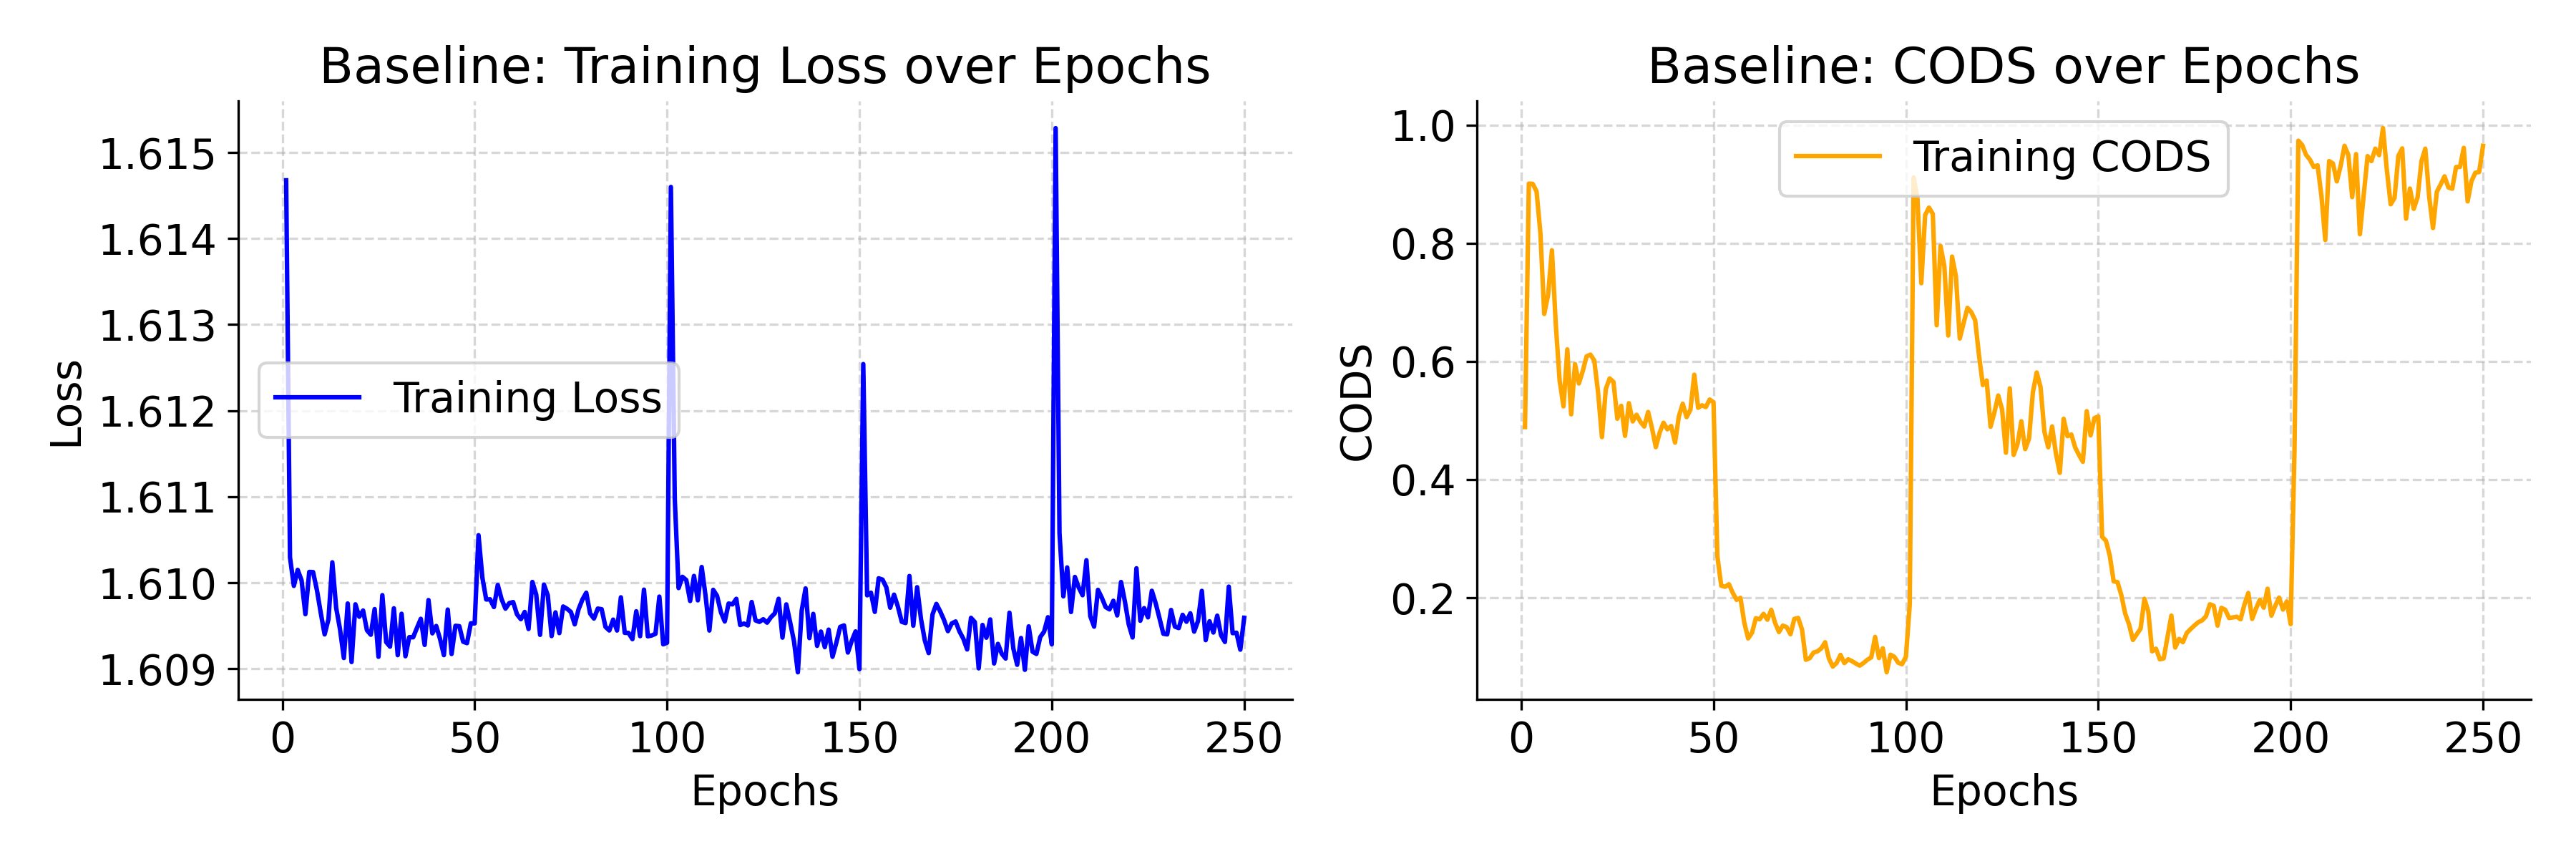
\includegraphics[width=\textwidth]{img/baseline_dropout_tuning.png}}
    \caption{Comparison of training loss and CODS across epochs for baseline dropout tuning.}
    \label{fig:loss_cods}
\end{figure}

Figure \ref{fig:ablations} displays ablation studies that assess the impact of sequence length and multiple training epochs on model outputs. These experiments reaffirmed that hyperparameter tuning plays a crucial role in stabilizing training and enhancing creative outputs.

\begin{figure}[h!]
    \centering
    \subfigure[Sequence Length Variation]{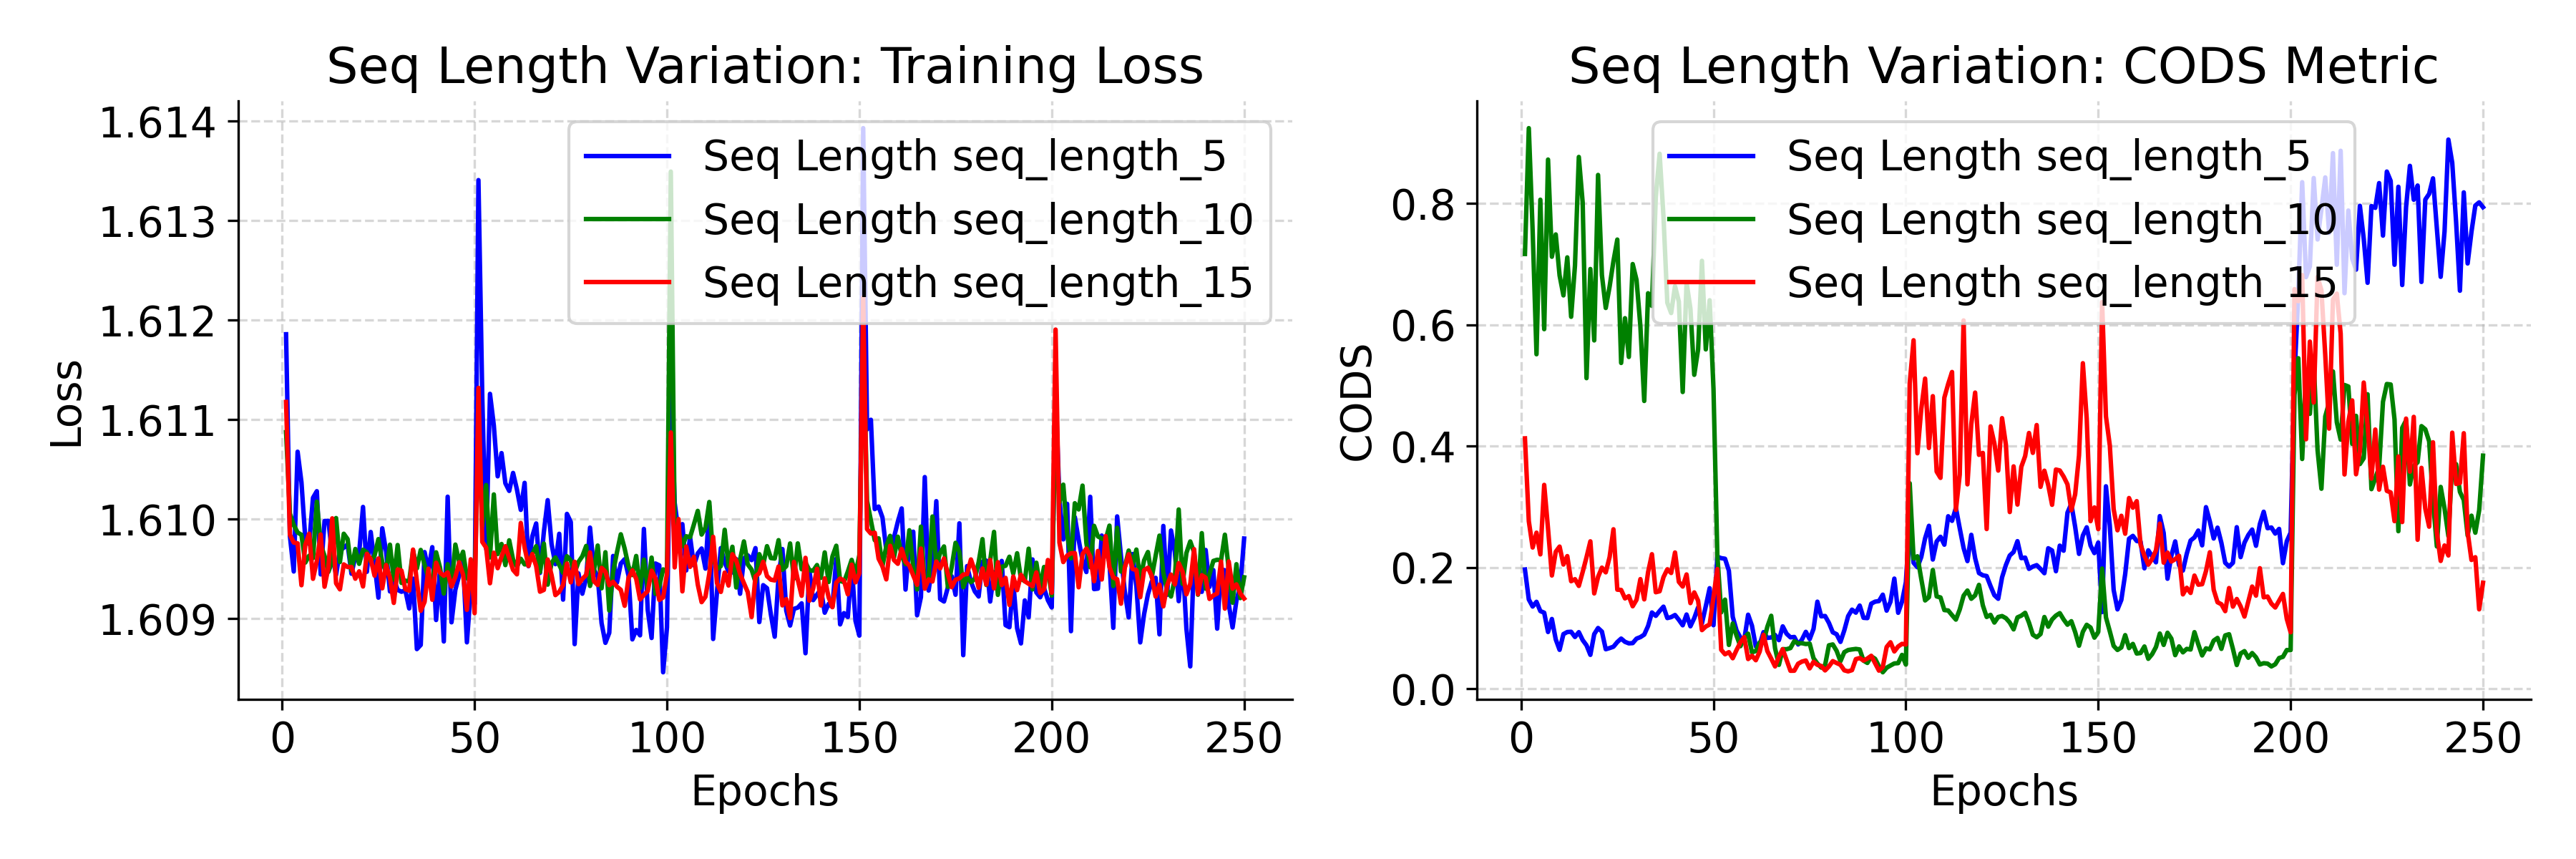
\includegraphics[width=\textwidth]{img/ablation_sequence_length_variation.png}}
    \hspace{0.5cm}
    \subfigure[Multiple Epochs Variation]{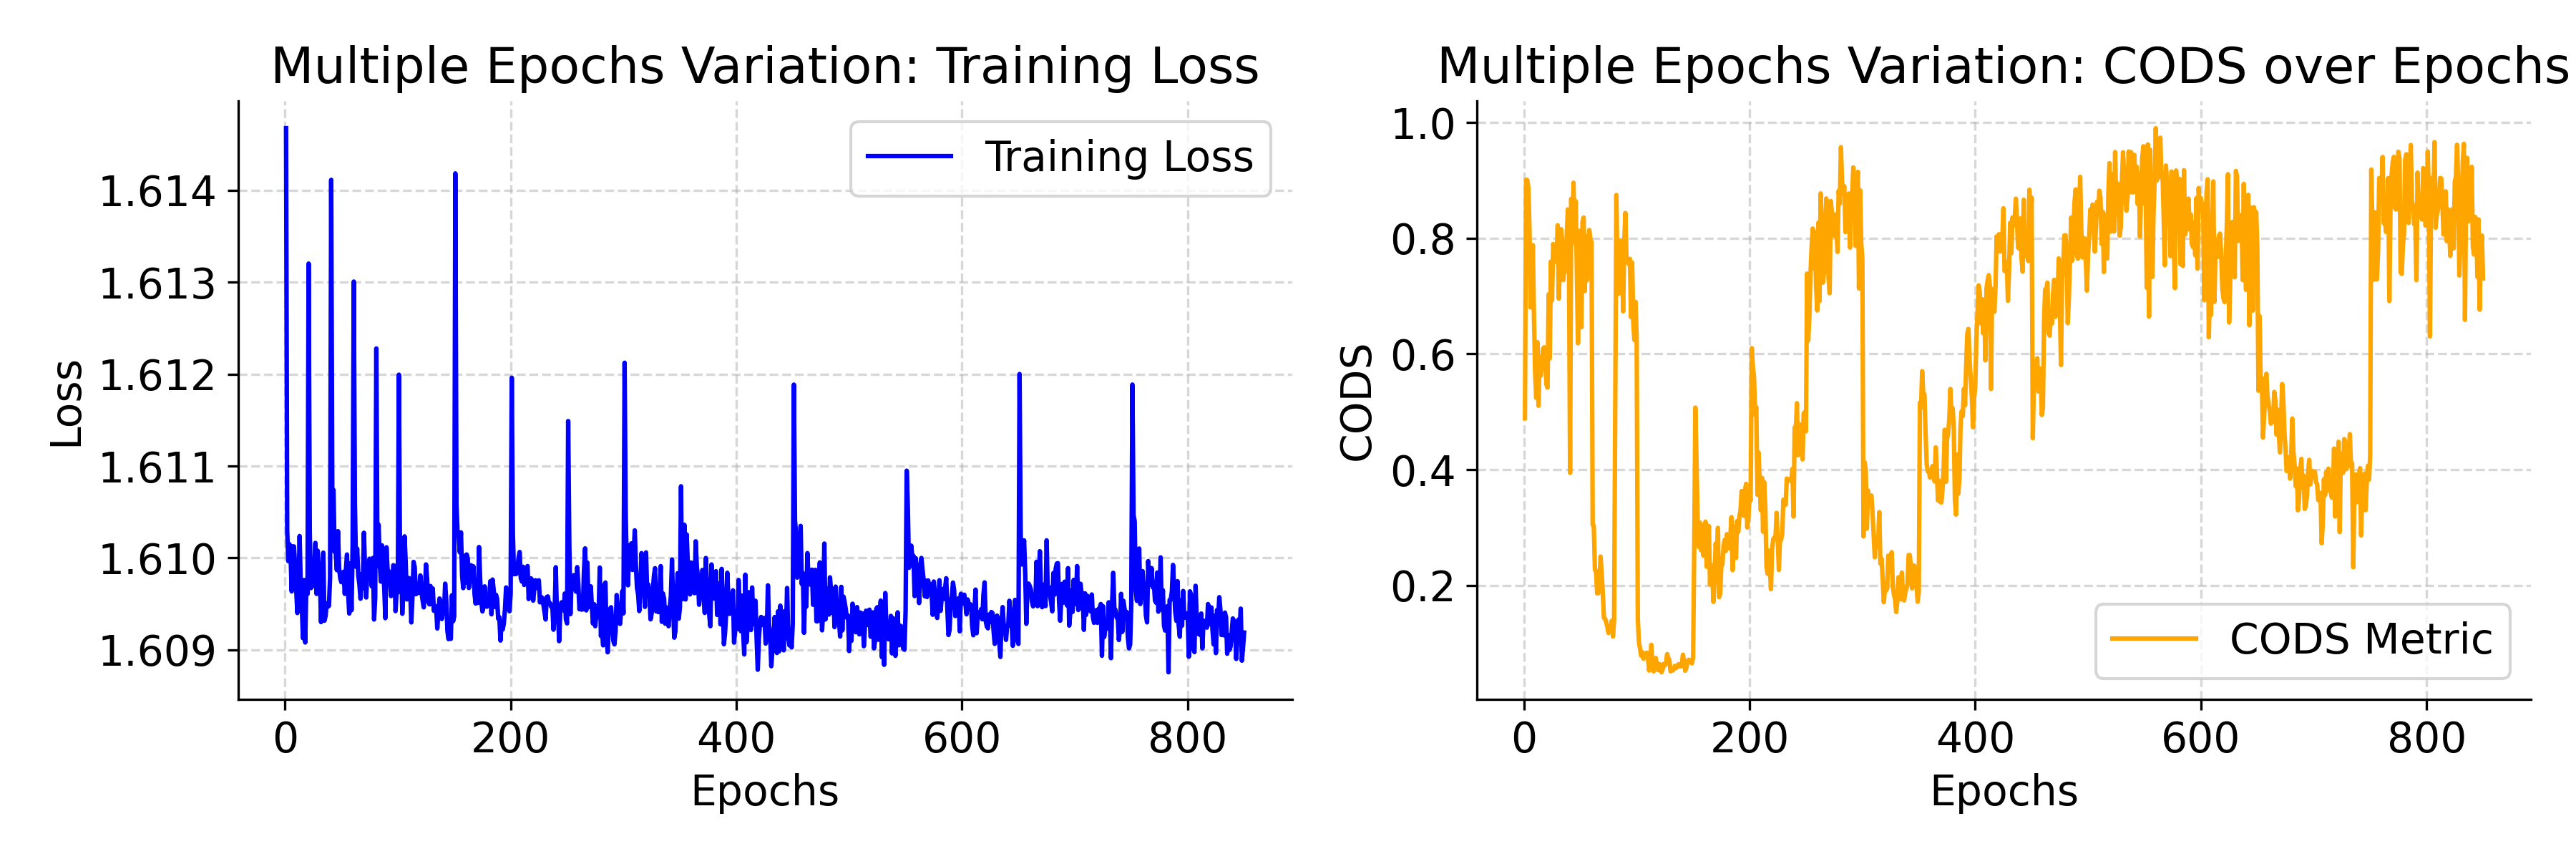
\includegraphics[width=\textwidth]{img/ablation_multiple_epochs_variation.png}}
    \caption{Ablation studies demonstrating the effect of sequence length and training epochs on model performance.}
    \label{fig:ablations}
\end{figure}

\section{Conclusion}
\label{sec:conclusion}
This research provides a comprehensive framework for assessing the creative capabilities of LLMs through MTP and seed-conditioning. Our findings highlight the importance of hyperparameter tuning and the impacts of training methodologies on model creativity. Future work will explore the application of these insights to broader real-world tasks, aiming to refine the balance between coherence and creativity in LLM outputs.


% \subsubsection*{Acknowledgments}
% Use unnumbered third level headings for the acknowledgments. All
% acknowledgments, including those to funding agencies, go at the end of the paper.


\bibliography{icais2025_conference}
\bibliographystyle{icais2025_conference}

% \appendix
% \section{Appendix}
% You may include other additional sections here.


\end{document}
